% Figura Anexo II: el mercado de trabajo con errores de predicción (FRIEDMAN 1968)
\documentclass[tikz,border=3pt]{standalone}
\usepackage[T1]{fontenc}
\usepackage[utf8]{inputenc}
\usetikzlibrary{arrows.meta,calc,positioning}
\begin{document}
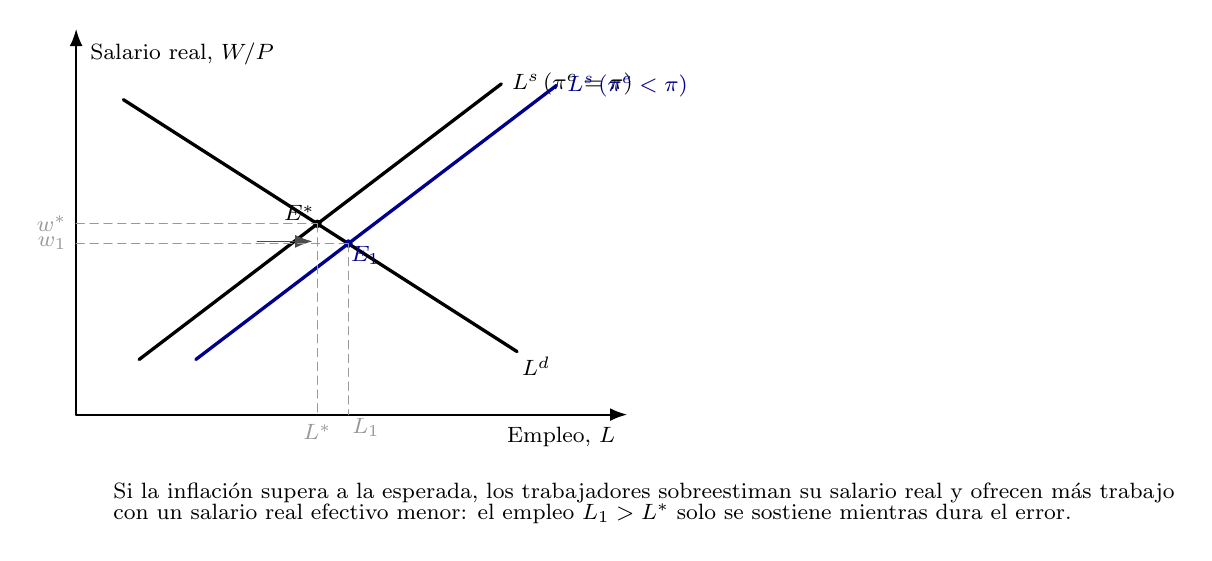
\begin{tikzpicture}[>={Latex[length=2.2mm]}, line cap=round, font=\footnotesize,
  eje/.style={->, thick},
  curva/.style={very thick},
  nueva/.style={very thick, blue!55!black},
  guia/.style={densely dashed, gray!80},
  pto/.style={circle, fill=black, inner sep=1.1pt}]
  \draw[eje] (0,0) -- (7.0,0) node[below left=1pt]{Empleo, $L$};
  \draw[eje] (0,0) -- (0,4.9) node[below right=2pt]{Salario real, $W/P$};
  % Demanda de trabajo (las empresas conocen su salario real)
  \draw[curva] (0.6,4.0) -- (5.6,0.8) node[below right=-3pt]{$L^{d}$};
  % Oferta con expectativas correctas
  \draw[curva] (0.8,0.7) -- (5.4,4.2) node[right]{$L^{s}\,(\pi^{e}=\pi)$};
  % Oferta con error de predicción (pi > pi^e): se desplaza a la derecha
  \draw[nueva] (1.52,0.7) -- (6.1,4.18) node[right]{$L^{s}\,(\pi^{e}<\pi)$};
  \draw[->, gray!60!black] (2.3,2.2) -- (3.0,2.2);
  \node[pto] (E0) at (3.064,2.423) {};
  \node[above left=-2pt of E0, inner sep=1pt] {$E^{*}$};
  \node[pto, fill=blue!55!black] (E1) at (3.457,2.172) {};
  \node[below right=-2pt of E1, inner sep=1pt, blue!55!black] {$E_1$};
  \draw[guia] (3.064,2.423) -- (3.064,0) node[below]{$L^{*}$};
  \draw[guia] (3.457,2.172) -- (3.457,0) node[below right=-3pt]{$L_1$};
  \draw[guia] (0,2.423) node[left]{$w^{*}$} -- (3.064,2.423);
  \draw[guia] (0,2.172) node[left]{$w_1$} -- (3.457,2.172);
  \node[align=left, anchor=north west] at (0.35,-0.75) {Si la inflación supera a la esperada, los trabajadores sobreestiman su salario real y ofrecen más trabajo\\[-2pt]con un salario real efectivo menor: el empleo $L_1>L^{*}$ solo se sostiene mientras dura el error.};
\end{tikzpicture}
\end{document}
